\documentclass[a4paper,oneside,phd,etd]{BYUPhys}
% The BYUPhys class is for producing theses and dissertations
% in the BYU Department of Physics and Astronomy.  You can supply
% the following optional arguments in the square brackets to
% specify the thesis type:
%
%   senior  : Produces the senior thesis preliminary pages (default)
%   honors  : Produces the honors thesis preliminary pages
%   masters : Produces the masters thesis preliminary pages
%   phd     : Produces the PhD dissertation preliminary pages
%
% The default format is appropriate for printing, with blank pages
% inserted after the preliminary pages in twoside mode so you can
% send it directly to a two-sided printer. However, for ETD
% submission the blank pages need to be removed from the final output.
% The following option does this for you:
%
%   etd     : Produces a copy with no blank pages in the preliminary section.
%             Remove this option to produce a version with blank pages inserted
%             for easy double sided printing.
%
% The rest of the class options are the same as the regular book class.
% A few to remember:
%
%   oneside : Produces single sided print layout (recommended for theses less than 50 pages)
%   twoside : Produces double sided print layout (the default if you remove oneside)
%
% The BYUPhys class provides the following macros:
%
%   \makepreliminarypages : Makes the preliminary pages
%   \clearemptydoublepage : same as \cleardoublepage but doesn't put page numbers
%                           on blank intervening pages
%   \singlespace          : switch to single spaced lines
%   \doublespace          : switch to double spaced lines
%
% --------------------------- Load Packages ---------------------------------

% The graphicx package allows the inclusion of figures.  Plain LaTeX and
% pdfLaTeX handle graphics differently. The following code checks which one
% you are compiling with, and switches the graphicx package options accordingly.
\usepackage{ifpdf}
\ifpdf
  \usepackage[pdftex]{graphicx}
\else
  \usepackage[dvips]{graphicx}
\fi

%%%%%%%%%%%%%%%%%%%%%%%%%%%%%%%%%%%%%%%%%%%%%%%%%%%%%%%%%%%%%%%%%%
% Edited : Beeshanga
%
% If you need to include any code in the text use this package
% \usepackage{listings}
% It can be used to make key words bold, add colours, etc. Refer
% to http://en.wikibooks.org/wiki/LaTeX/Packages/Listings for
% more information.
%
% For theorems, propositions, proofs and assumptions use this
% package
% \usepackage{amsthm}
% For more information refer to the following website
% http://en.wikibooks.org/wiki/LaTeX/Theorems
%
%%%%%%%%%%%%%%%%%%%%%%%%%%%%%%%%%%%%%%%%%%%%%%%%%%%%%%%%%%%%%%%%%%

% The fancyhdr package allows you to easily customize the page header.
% The settings below produce a nice, well separated header.
\usepackage{fancyhdr}
  \fancyhead{}
  \fancyhead[LO]{\slshape \rightmark}
  \fancyhead[RO,LE]{\textbf{\thepage}}
  \fancyhead[RE]{\slshape \leftmark}
  \fancyfoot{}
  \pagestyle{fancy}
  \renewcommand{\chaptermark}[1]{\markboth{\chaptername \ \thechapter. #1}{}}
  \renewcommand{\sectionmark}[1]{\markright{\thesection \ #1}}


% The cite package cleans up the way citations are handled.  For example, it
% changes the citation [1,2,3,6,7,8,9,10,11] into [1-3,6-11].  If your advisor
% wants superscript citations, use the overcite package instead of the cite package.
\usepackage{cite}

% The makeidx package makes your index for you.  To make an index entry,
% go to the place in the book that should be referenced and type
%  \index{key}
% An index entry labeled "key" (or whatever you type) will then
% be included and point to the correct page.
%\usepackage{makeidx}
%\makeindex

% The url package allows for the nice typesetting of URLs.  Since URLs are often
% long with no spaces, they mess up line wrapping.  The command \url{http://www.physics.byu.edu}
% allows LaTeX to break the url across lines at appropriate places: e.g. http://www.
% physics.byu.edu.  This is helpful if you reference web pages.

\usepackage[hyphens]{url}
\urlstyle{same}
\usepackage{cite}

%\usepackage{url}
%\urlstyle{rm}

% If you have a lot of equations, you might be interested in the amstex package.
% It defines a number of environments and macros that are helpful for mathematics.
% We don't do much math in this example, so we haven't used amstex here.
\usepackage{amsmath}
\usepackage{amssymb}
\usepackage{subfigure}
\usepackage{cite}
\usepackage{amsxtra}
\usepackage{amsfonts}
\usepackage{graphicx}
\usepackage{multirow} % This is package for multi-rows in tables added on 7th July 2009 by Arif
%\usepackage{setspace}

% The caption package allows us to change the formatting of figure captions.
% The commands here change to the suggested caption format: single spaced and a bold tag
\usepackage[labelfont=bf,labelsep=colon]{caption}%[2008/04/01]
 \DeclareCaptionFormat{suggested}{\singlespace#1#2#3\par\doublespace}
 \captionsetup{format=suggested}


\usepackage{array}
\usepackage{multirow}
\usepackage{verbatim}
\usepackage{enumerate}

% Defining the symbols




% The hyperref package provides automatic linking and bookmarking for the table
% of contents, index, equation references, and figure references.  It must be
% included for the BYU Physics class to make a properly functioning electronic
% thesis.  It should be the last package loaded if possible.
%
% To include a link in your pdf use \href{URL}{Text to be displayed}.  If your
% display text is the URL, you probably should use the \url{} command discussed
% above.
%
% To add a bookmark in the pdf you can use \pdfbookmark.  You can look up its usage
% in the hyperref package documentation
\usepackage[bookmarksnumbered,pdfpagelabels=true,plainpages=false,colorlinks=true,
            linkcolor=black,citecolor=red,urlcolor=blue]{hyperref}
\hypersetup{breaklinks=true}

% My custom packages
\usepackage{float}
\usepackage{parskip}


% ------------------------- Fill in these fields for the preliminary pages ----------------------------
%
% For Senior and honors this is the year and month that you submit the thesis
% For Masters and PhD, this is your graduation date
  \Year{2019}
  \Month{June 7th,}
  \Author{James Ridey}

% If you have a long title, split it between two lines. The \TitleBottom field defines the second line
% A two line title should be an "inverted pyramid" with the top line longer than the bottom.
  \TitleTop{Matrix multiplication through}
  \TitleBottom{stochastic numbers} % edited Beeshanga
 \DegreeTitle{Bachelor of Engineering
 \\ Software Engineering} % edited Beeshanga

% Your research advisor
 \Advisor{Supervisor: Associate Professor Tara Hamilton}

% The department undergraduate research coordinator
%  \UgradCoord{A}

% The representative of the department who will approve your thesis (usually the chair)
%  \DepRep{B}

% Acknowledge those who helped and supported you

  \Acknowledgments{
  \vspace{-1.5cm}
    \noindent I would like to acknowledge and thank, Tara Hamilton and Alan Kan for their support and advice during my thesis.
  }


% The title of the department representative
%  \DepRepTitle{Chair}
  \Statement{
    \noindent I, James Ridey, declare that this report, submitted as part of the requirement for the award of Bachelor of Engineering in the School of Engineering, Macquarie University, is entirely my own work unless otherwise referenced or acknowledged. This document has not been submitted for qualification or assessment at any academic institution.
    \vspace{0.5cm}

    \noindent     Student's Name: James Ridey

    \vspace{0.25cm}

    \noindent Student's Signature: James Ridey

    \vspace{0.25cm}

    \noindent     Date: 7/6/2019
    }

% The text of your abstract
\Abstract{
\vspace{-1.5 cm}
Neural networks are considered a core foundation of machine learning and has recently ballooned into a large framework that requires vast amounts of computing resources and time. 
Here, we examine how to improve the efficiency of these networks, by utilizing ideas such as stochastic numbers and probabilistic results to reduce the overall training time and/or the consumption of computing resources.
As such a core part of machine learning networks is a matrix multiplication and implementing this operation in stochastic numbers would be a first step to trying to use stochastic numbers within the domain of machine learning.
}



% Statement of Candidate



\fussy

\begin{document}

 % Start page counting in roman numerals
 \frontmatter

 % This command makes the formal preliminary pages.
 % You can comment it out during the drafting process if you want to save paper.

 \makepreliminarypages


%\clearemptydoublepage
\doublespace
%\include{Publications/publications}

% \clearemptydoublepage
%\include{Organization/organization}

 \clearemptydoublepage
\singlespace
 % Make the table of contents.
 \tableofcontents

\clearemptydoublepage
% Make the list of figures
\listoffigures

\clearemptydoublepage
% Make the list of tables
%\listoftables

\clearemptydoublepage

% Start regular page counting at page 1
\mainmatter
%
\chapter{Introduction}
\label{chap:Introduction}


\section{Neural networks: Introduction}
Neural networks are the core structure of what many believe to be the next step in computing, machine learning. We are starting to see machine learning used to solve problems that originally were only able to be solved by people\cite{bojarski2016end}. However, all this machine learning comes at a cost, machine learning needs vast amounts of data to learn and thus large amounts of computing resources, electricity, time and even the best machine learning models work within a narrow, controlled set of inputs, anything outside this "range" are misclassified, in other words, machine learnings models are sensitive to noise and not general enough.

In my preliminary thesis, I detailed how machine learning models react to noise and shared some of my initial tests, in this final thesis we try to expand and implement a matrix multiplication, a core component of neural networks through the use of stochastic numbers.

\chapter{Background and Related Work}
\label{chap:LitReview}


\section{Neural networks: introduction}
Neural networks are the core structure of what many believe to be the next step in computing, machine learning. We are starting to see machine learning used to solve problems that originally were only able to be solved by people. However, all this machine learning comes at a cost, machine learning needs vast amounts of data to learn and thus large amounts of computing resources, electricity, time and even the best machine learning models work within a narrow, controlled set of inputs, anything outside this "range" are misclassified, in other words, machine learnings models are sensitive to noise and not general enough.

\section{Project goal}
My thesis project goal is primarily trying to reduce neural network complexity. Complexity that forms due to the vast amount of data that needs to be worked through and the finicky nature of neural networks. Overall I've identified an avenue that I plan to explore in more detail: creating an alternative neural network model using stochastic numbers. With the goal of this model to be more efficient in computational time and/or being able to train faster while still maintaining the same levels of accuracy.

\chapter{Background and Related Work}
\label{chap:LitReview}

\section{Neural networks: explanation}
Neural networks are a very rough simulation of how the neurons in a human brain actually work\cite{neural-network-intro}, they have been researched since the 1960s\cite{neural-network-history} but at the time we did not have the computing power necessary to run these large neural networks and thus progress was halted until around 1970-1980's when backpropagation was discovered making neural network training much more efficient and parallel computing system was also starting to kick off.

The most common form of a neural network in the feedforward model where the inputs are passed to the neural network and it outputs an answer. The feedforward model consists of an input layer, hidden layers and an output layer. Each of these layers are composed of varying amounts of neurons depending on the complexity of the data that is trying to be learned. More models of neural networks exist which aim to memorise or improve the feedforward model, however, the feedforward model is incredibly ubiquitous and is the main driving force behind machine learning in the industry. 

To understand what each layer in a neural network is doing, it is first necessary to understand what a neuron is doing. A neuron is comprised of inputs, a set of weights, one output and an activation function\cite{neural-network-intro-book}, as shown below.
\begin{figure}[H]
\centering
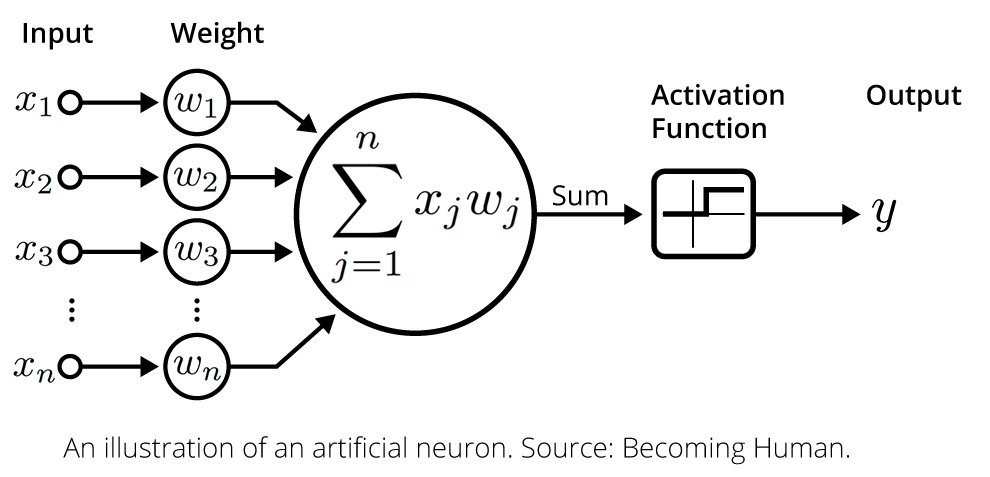
\includegraphics[width=8cm]{pictures/neuron_model.png}
\caption{Neuron model\cite{fig:neuron_model}.}
\label{fig:neuron_model}
\end{figure}

Neurons are fed a set of data through its inputs which are multiplied by a specific weight, all of these numbers are then added up and fed to an activation function. An activation function is a function that maps the input to a value between 0 and 1, a commonly used activation function is the sigmoid function, numbers in the positive infinity direction become increasingly closer to 1, while numbers in the negative infinity direction become increasing closer to 0.
\begin{figure}[H]
\centering
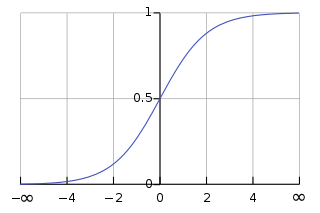
\includegraphics[width=8cm]{pictures/sigmoid.png}
\caption{Sigmoid graph\cite{fig:sigmoid}.}
\label{fig:sigmoid}
\end{figure}

The next concept is neural network layers which vary based on the task you want to try an accomplish, some examples include convolutional layers which attempt to use neural networks on squares of pixels, dropout layers which randomly pick weights to drop to try and reduce overfitting and the most common layer used to most machine learning models, is the dense layer. In this layer, every neuron connects to every other neuron in the previous layer.
\begin{figure}[H]
\centering
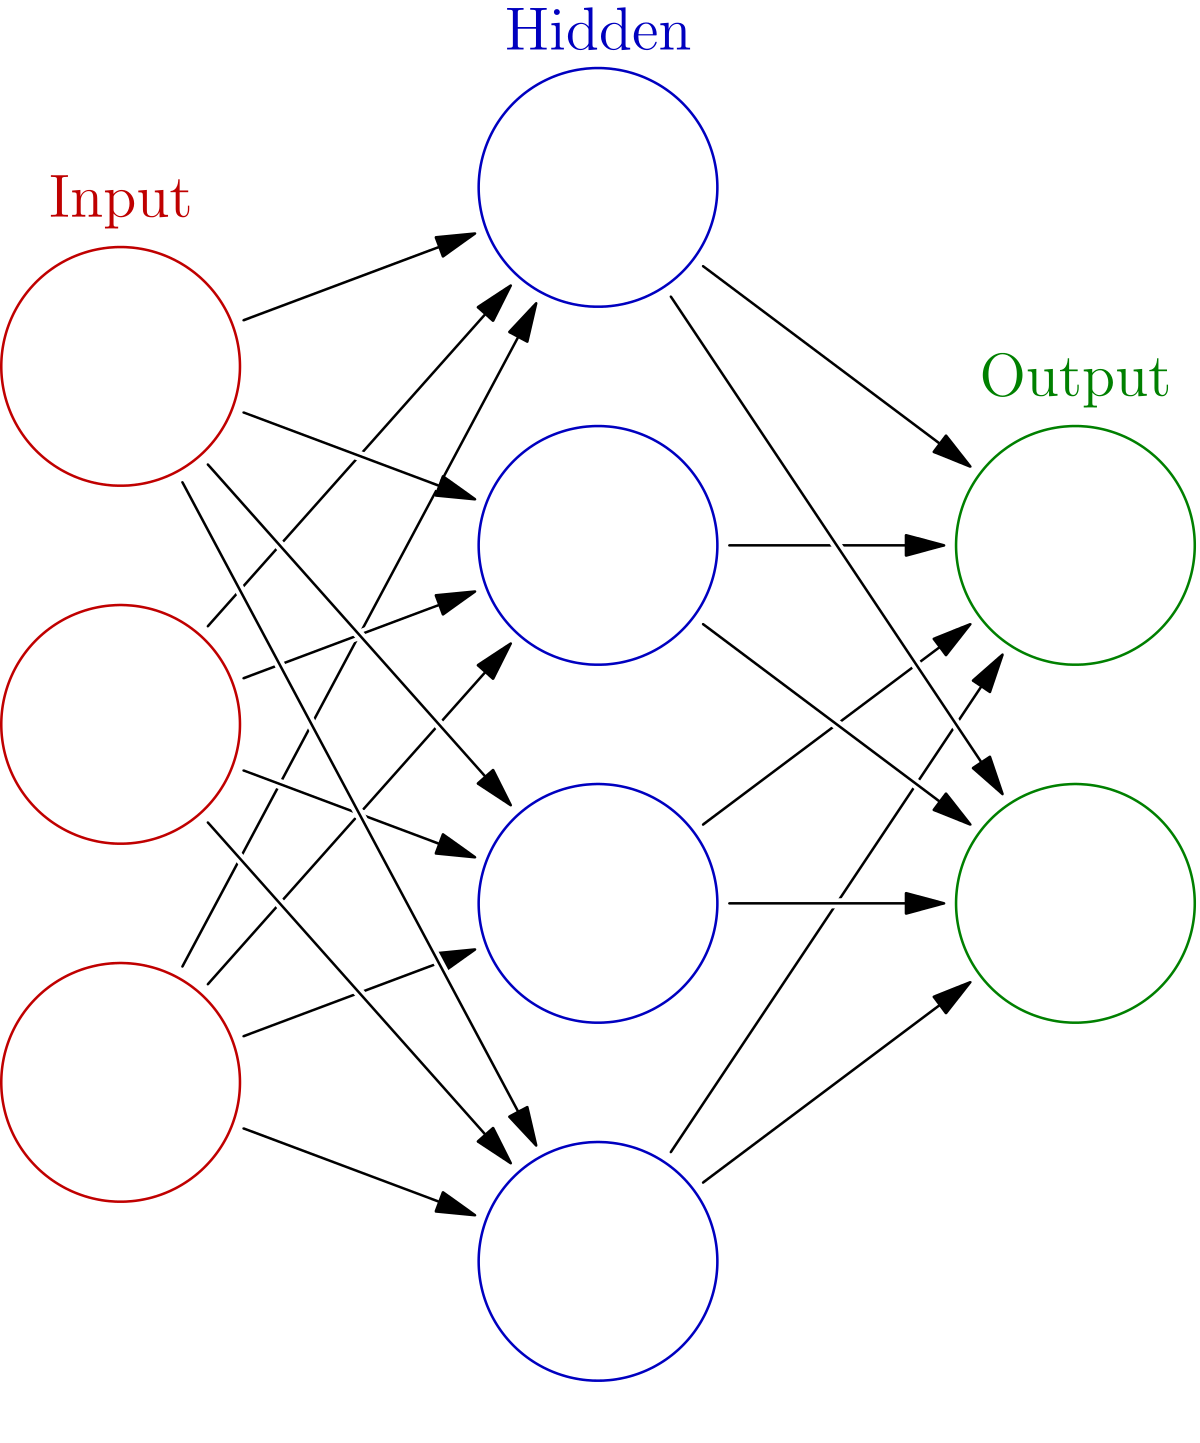
\includegraphics[width=8cm]{pictures/neural_network_model.png}
\caption{Dense layer neural network model\cite{fig:neural_network_model}.}
\label{fig:neural_network_model}
\end{figure}

Each circle in this figure represents a neuron and each line in this figure represents a connection between 2 neurons. By manipulating the weights in the neural network, we change what each neuron calculates and outputs as part of its activation function. In doing so, we now have a framework of which for any given input, the neural network can generate any output (given the right weights), regardless of the complexity of the output\cite{nielsen}. 

\subsection{Training}
The next question about neural networks is then how are the weights calculated for a given input. This is where training a neural network comes into play. The basic summary for how a neural network is trained is they are fed the input data, the error amount is calculated from the difference between the neural network output and the expected output. Then the weights are slowly adjusted to minimize the error rate. How this is all done is where the complexity of neural networks lie and why they take so long to train. One of the simplest algorithms that implements this is the stochastic gradient descent algorithm, which is a core component of many other machine learning algorithms like RMSprop, ADAM and AdaGrad (RMSprop being a commonly used algorithm and the one that was used in the majority of the MNIST tests). 

The gradient descent or GD works by measuring the gradient and trying to find a point at which the error is the lowest. The gradient being a measure of "how much the output of a function changes if you change the inputs a little bit"\cite{towards-data-science}.
The best way of explaining GD is with a hill-climbing example, a blind person is trying to find the highest point of a hill and so he starts by taking large steps to estimate where the steepest part of the hill is and then smaller and smaller steps until he finds the top of the hill. Applying this to machine learning, the error of the output of the machine learning model is compared with the actual values that are to be expected and this is the error amount, then the weights are changed are relatively "large" amount and the error is measured again and compared to the previous error, this is the gradient. This gradient is then used to estimate how big of a "step"/how much to adjust the weights by on the next iteration.
\begin{figure}[H]
\centering
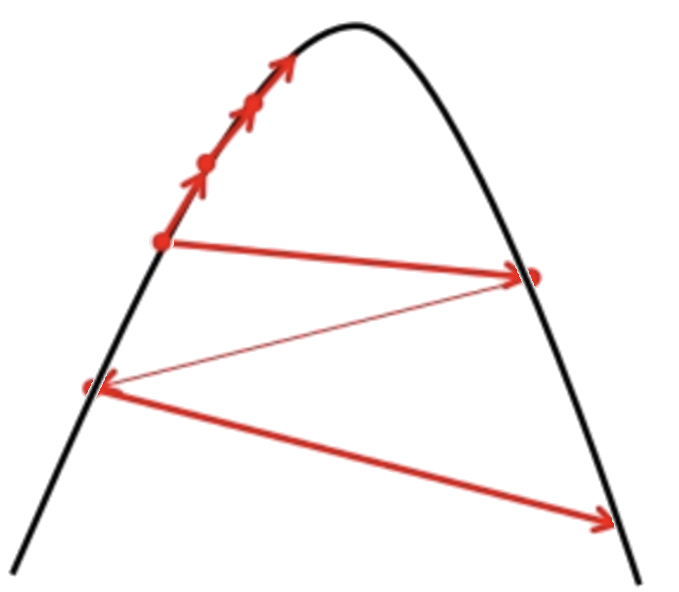
\includegraphics[width=6cm]{pictures/gradient.png}
\caption{Stochastic gradient example.
Y-Axis represents accuracy rate}
\label{fig:gradient}
\end{figure}

However in realities, there are much more dimensions to a machine learning model and secondly, there is not just one point that is the highest but multiple hills of varying heights, this is one of the many reasons why machine learning is hard. You can create simple machine learning algorithms that find a maximum point but not the global maximum point or the global maxima, you can also try and adjust how much you step by each amount but the best way, which requires all the computation power is a small stepping amount which tries all points on the "hills". 
\begin{figure}[H]
\centering
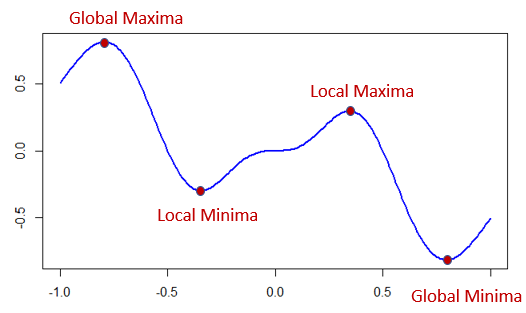
\includegraphics[width=10cm]{pictures/global_minima.png}
\caption{Global maxima example.
Y-Axis represents accuracy rate}
\label{fig:global_minima}
\end{figure}

\section{Complexities of neural networks}
The main question about this thesis is what makes training neural networks so computationally complex, why neural networks are trained through large GPU farms and the challenges facing researching trying to shrink the size of these neural networks.

\subsection{Overfitting and underfitting}
Neural networks are a statistics tool with the main purpose of being able to generalize from one set of training data and then predict a value based on a new set of input data. 

To train a neural network, we divide the training into 2 phases, the learning/training stage and the prediction state. The learning/training stage is where the weights of the neural network are adjusted using backpropagation or a similar algorithm and the neural network is trying to fit the data as well as it can by correctly predicting the correct value for each given input. Then the prediction stage is where the neural network is evaluated against a subset of the data that it has not seen before, this stage is purely to combat overfitting\cite{overfitting}.

Overfitting is when the neural network begins to fit so well with the training data, that is unable to generalise/achieve good accuracy in the prediction stage. In other words, it fails as a classification or prediction model because it hasn't really learnt the underlying structure of the data but rather is just "cheating" in the training stage.

Conversely, underfitting occurs when the neural network fails to achieve any accuracy in the training or prediction stage, this is quite rare to see in practice but can occur with bad datasets or a too simplistic neural network model\cite{underfitting-machine-learning}.

\subsection{Complexities}
Given overfitting and underfitting, it becomes a challenge to train neural networks because having a model that is too simplistic will cause underfitting and having a model that is too large not only increases computation time with all the various amounts of weights that each layer incurs but also leads to overfitting\cite{model-complexity}. 

Not to mention, the training stage usually requires multiple iterations and the backpropagation algorithm has a high time complexity\cite{backprop-time-complexity}. All in all, this means we end up with a large neural network, with thousands to millions of weights and due to how neural networks work, most of the operations needed are matrix multiplications which is what GPU's tend to be good at, considering computer graphics are just matrix manipulations.

\section{Research into neural network complexity}
There has been a lot of research in neural networks, while much of it is focused upon learning more and more complex datasets\cite{research-1}\cite{research-2}\cite{research-3}, there has also been a lot of research into trying to prune neural networks and a large number of parameters (weights) that are needed for these large scale neural networks. A recent example is "Importance Estimation for Neural Network Pruning"\cite{molchanov2019taylor}, where they cite a 40\% reduction in complexity by trimming off 30\% of the parameters.

In the field, which I'm planning to research there have been a few papers on stochastic numbers and the benefits regarding using them on neural networks, for example, one such paper states a 47\% area and 60\% power reduction while maintaining a high accuracy rate\cite{8119196}. 

Another paper\cite{7093194} goes on to show how its stochastic neural network allows for building reliable systems due to the high level of noise-immunity that the network model shows.

While both of these papers are impressive research and they show that their networks are comparable with a regular dense layer neural network or MLP (Multi-Layer Perceptron) for short, they fail to address advantages and disadvantages that a stochastic neural network might bring to the table, an example of such an advantage is how a stochastic neural network compares with a regular MLP network when exposed to a noisy dataset. The previous paper regarding noise immunity is mainly focused around random noise injected alongside the input data, not noise inherent within the input data. One of my research avenues is to explore how stochastic neural networks, react to noise during the training and validation stages.

\section{Matrices in neural networks}
One of the important things to understand about a neural network is how they are implemented, this will help when discussing how stochastic computing could potentially help with neural networks. The core component of almost all machine learning frameworks and neural networks is the matrix multiplication operation, this is used during the feed-forward operation of the network, computing the output for each of the inputs and the weights of each layer.

Since each layer is composed of neurons which take all the inputs and multiplies it with all of the weights, it is functionally identical to a matrix multiplication where the first matrix is the inputs to the neural network layer, the second matrix is the weights of that layer and the output matrix is the output of the current layer.
\begin{figure}[H]
\centering
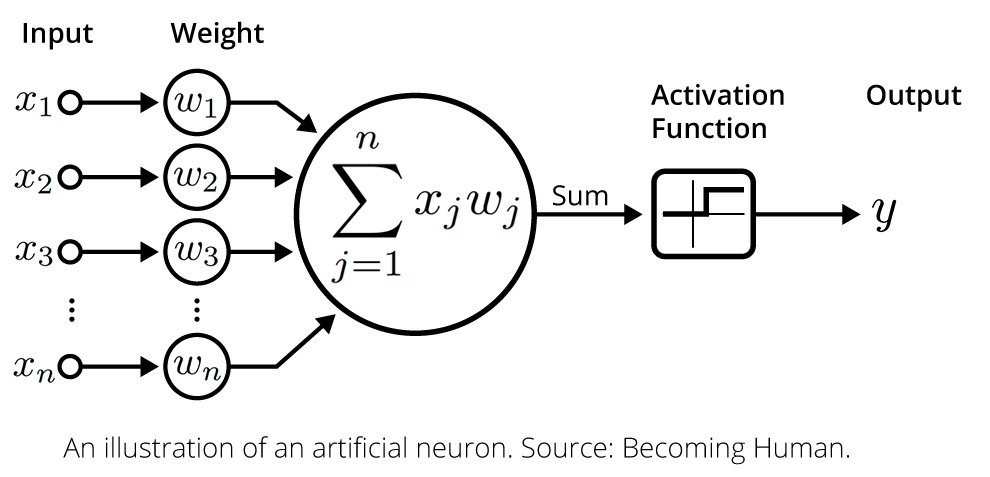
\includegraphics[width=8cm]{pictures/neuron_model.png}
\caption{Neuron model\cite{fig:neuron_model}.}
\label{fig:neuron_model}
\end{figure}
\begin{figure}[H]
\centering
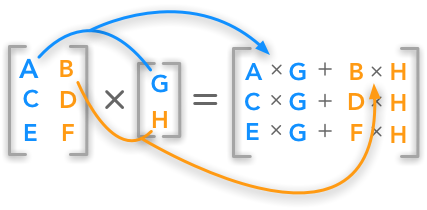
\includegraphics[scale=0.5]{pictures/matrix-multiply.png}
\caption{Matrix multiplication\cite{fig:matrix-multiply}.}
\label{fig:neuron_model}
\end{figure}
What advantage can we get out of neural networks being represented this way? The major advantage is that the component responsible for rendering graphics on the computer, the GPU is extremely efficient at matrix multiplications partially because of the architecture is arranged for bandwidth instead of latency, partially because GPU's have multiple cores that run in parallel and mostly because 3D graphics are all about matrix multiplications to map 3D points to 2D through a camera matrix.

\section{Stochastic computing}
Stochastic computing is a branch of computing that relies on probabilistic bitstreams to calculate numbers, often relying on simple bit-wise operations. Every number in a stochastic computer is arranged as a probability of the ones and zeros in a continuous binary number stream\cite{6800290}. 

\subsection{Advantages of stochastic numbers}
There are 2 major advantages with this technique, one is that the system is extremely resistant to noise\cite{8122049}, flipping multiple bits in the stream will have very little effect or will only change the number minorly. The other major advantage is that certain operations have a simpler solution, for example in terms of multiplication on a conventional computer this would be a $n^2$ operation, however, on a stochastic computer, this is accomplished with an AND gate at a cost of $O(n)$.

\subsection{Disadvantages of stochastic numbers}
However, the reason for stochastic computing not being proliferated is the inherent weakness which is the randomness of stochastic numbers. Stochastic numbers can never truly represent the number they are trying to calculate and thus need a large amount of sampling to produce a more accurate result, they simply try to "emulate" a floating point number by using the ratio of 1's and 0's as a probability.

Secondly is that while stochastic numbers have a simple analog for multiplication, the core of stochastic numbers like the PRNG (Pseudo-random number generator) for generating the random bitstream and decoding the bitstream by sampling do not have simple gate-level analogues and this is where stochastic numbers lose their advantage.

%\section{Research into stochastic numbers}
%TODO

\section{Machine learning frameworks}
Both Tensorflow and PyTorch were used to emulated stochastic computing inside of a machine learning system, however, due to complications that arose when trying to implement the stochastic operations this was ultimately scrapped and the results found in this thesis were made using Python 3.

\section{Tensorflow}
Tensorflow\cite{tensorflow} is a machine learning framework primarily written in Python. It was released by Google under the Apache License 2.0 on November 9th, 2015. The Tensorflow network employs the idea of creating a neural network model which is then compiled before being handed off to the appropriate processing unit be it CPU, GPU or TPU, this is in contrast to other machine learning frameworks like PyTorch that generate their models dynamically on the fly which results in a small performance hit.

Tensorflow continues to grow in support with new frameworks like Kera that aim to simplify common operations and overall streamline the process and show no signs of stopping with a stable release only 2 months ago.

\section{PyTorch}
PyTorch\cite{pytorch} is another machine learning framework that is also written in Python, it is primarily developed by Facebook under a modified BSD license, first released in October 2016. PyTorch offers similar benefits to Tensorflow with easy GPU and CPU optimization as well as premade Dense, RNN and CNN networks, furthermore, as the thesis progressed, it became apparent that Tensorflow was not a suitable framework to do low-level operations such as trying to implement the matrix multiplication with stochastic numbers. PyTorch fixes this issue by working at a much lower level than Tensorflow that allows direct access to its feed-forward and backpropagation components, it also allows users to directly define their networks and how they should be computed.

\section{The Idea}
To help understand this concept, it is important to explain the origin of this idea of using stochastic numbers for machine learning. One of the underlying issues with neural networks is that they are slow and are sensitive to noise in the dataset. An idea to speed them up and to make them more noise resistant, mainly comes from spiking neural networks. Spiking neural networks are built on the idea of artificial spiking neurons which are meant to be much more analogous to a human neuron, instead of matrix multiplications and activation functions, a spiking neuron is a neuron that takes in a stream of spikes of activity and after a certain threshold of spikes outputs its own spike, creating a so called spike train. Stochastic numbers act in a similar way, you have spikes (1's) in a bitstream of information and process them in some way to get more or fewer spikes. Stochastic numbers are known to have properties that would make them beneficial in neural networks such properties include noise resistance and faster floating point operations.

So the idea was to see how stochastic numbers would work in a machine learning domain and the first step to this would be to replicate what a regular neural network model does which is a series of matrix multiplications.
\begin{figure}[H]
\centering
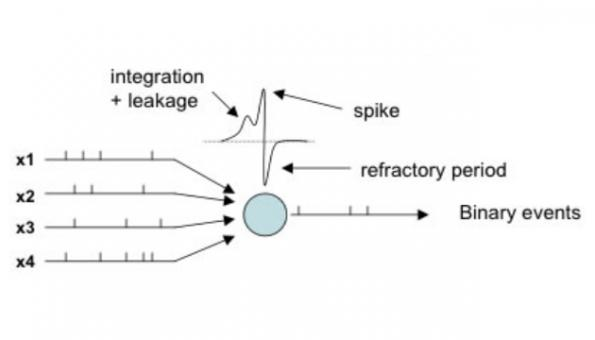
\includegraphics[scale=0.5]{pictures/spikingneuron.jpg}
\caption{Spiking neuron\cite{fig:spiking-neuron}.}
\label{fig:neuron_model}
\end{figure}


\chapter{Implementation}
\section{Introduction}
The primary idea behind this thesis was to create a system where we could reliably compare 2 machine learning systems with one using stochastic computing and the other using conventional computing. While attempts have been made in building up entirely new systems from the ground up using stochastic computing to accomplish a machine learning task\cite{hirtzlin2019stochastic}. As far as the research shows there have been little to no systems that use stochastic computing inside of existing machine learning framework such that both systems are on an even playing field and you aren't comparing oranges and apples. This was the goal we set out to accomplish, creating a system within an existing machine learning framework that could be applied to multiple datasets.

\section{The design}
Considering that the goal of this thesis was to compare stochastic computing and conventional computing in the field of machine learning, the first step would be to implement the core part of a machine learning framework which is the matrix multiplication, this consists of three parts, the conversion from a binary floating-point number to a stochastic number, the multiplication between the rows and columns of the matrix and finally the addition of each of the rows of the matrix. While most of these operations would be easy outside of a machine learning framework, implementing them within a machine learning framework requires a different way of thinking as each operation needs to be parallelizable and as such you are often restricted with what you are "allowed" to do, one such example of this is the heavy discouragement of the use of for loops\cite{broadcasting} as used incorrectly this requires the data being processed to be passed between the GPU and CPU and will likely cause massive slowdowns.

Each task had multiple ways of implementing the solution and each came with their benefits and drawbacks, which is expanded in more detail below.

\section{The conversion}
One of the secondary goals of this project was to create essentially a drop-in machine learning layer that would use stochastic computing, this would mean that the drop-in would have to convert the floating points it had received from the previous layer, convert it to a stochastic number for processing and then convert it back after the computation.

The general operation for how a binary number is converted to a stochastic number is 
\begin{enumerate}
	\item Create a boolean array the size of the stochastic number you want
	\item For each boolean in the array, set it to the condition (value $\geq$ random\_float(0,1))
\end{enumerate}
This is further shown in the Python code below
\begin{verbatim}
stochastic_num = [1 if random.random() <= prob1 else 0 for n in range(length)]
\end{verbatim}
However in terms of a machine learning framework the following is done instead, 
\begin{enumerate}
	\item Take the matrix of floating points, and add an extra dimension to it
	\item Scale the size of the newly created dimensional such that it repeats each value for the size of the stochastic number
	\item Apply (value $\geq$ random\_float(0,1)) over the entire matrix
\end{enumerate}

This covers the general approach to converting binary numbers to stochastic numbers, converting them back means simply taking the mean of the entire array/matrix. However, while this covers the general approach some nuances need to be discussed. The first is the use of the random number generator, stochastic numbers are very sensitive to correlation\cite{8342234} and so each random number must be generated separately from the other, while a general pseudorandom number generator (PRNG) will certainly do the trick, there have been studies showing better results can be achieved with a customised PRNG\cite{lee2019synthesizing}, we decided against going down this route as it would be complicated to integrate and ultimately detract from the goal of this thesis.

Another nuance of this algorithm is the size of the stochastic number, having more bits in your stochastic number will ultimately improve its performance but it comes at the cost of memory (which can balloon very quickly with large matrixes) and computational time. Plus after further investigation, we found that increasing the number of bits has diminishing effects.

As shown in the graph above, as the bits increase, the variance decreases but it reaches a point where the number of bits accounts for such a small change in the variance that it is ultimately not worth the memory or time. We did some research to try and find a way to have progressive accuracy with stochastic computing but we unable to find any instances of such a case. And finally the last nuance is the range of the stochastic numbers as the conditional (value $\geq$ random\_float(0,1)) will give a range on the stochastic numbers between 0 and 1, there exists an alternative form for negative numbers where the conditional becomes (value+1/2 $\geq$ random\_float(0,1) essentially the -1 to 1 range of value is mapped between 0 and 1. 

However there are a few caveats with this, one is that now each bit of the stochastic number represents a larger range and thus you need a large number of bits to accurately represent a number with a large number of digits after the decimal point, the second problem is that numbers can become small enough that when represented in a stochastic format they essentially become zero and no longer have an impact on the final value when they might have had a small but meaningful impact on the final value if they were not being computed stochastically. 

\section{Format}
For stochastic numbers, there are 2 main formats in which they can be represented with each format changing how results are calculated. The first most common format is the unipolar format in which each bit in the stochastic bitstream has a probability of $\frac{1}{number\ being\ represented}$ this in turn only allows the stochastic bitstream to have a range from 0 to 1, with 0 being where all the bits are 0's and 1 being where the entire bitstream is composed of 1's. As a quick example $X = SN 1000111010111001$, this stochastic bitstream would represent the number $X = 0.5625$ as there are 9 one's with a length of 16 ($\frac{9}{16} = 0.5625$)

The other format is the bipolar format in which each bit in the bitstream is represented by the probability of $\frac{number\ being\ represented-1}{2}$, the advantage with this format is the range is expanded out to (-1,1). While in a unipolar format each 1 and 0 represent a positive range, zero's represent -1 and one's represent 1, this means that a unipolar stochastic bitstream that is equal to 0 is composed of half 1's and half 0's. As example of bipolar bitstream, $X = BSN 1100110100000100$, this stochastic bitstream would represent the number $X = -0.25$ as there are 6 one's and 10 zero's with the length being 16 ($\frac{(+6) + (-10)}{16} = -0.25$)

While each format can easily be multiplied to a larger range once converted back to a floating-point number, what matters is how certain operations like multiplication differ between unipolar and bipolar. In multiplication for unipolar stochastic numbers, we use the AND gate and for bipolar stochastic numbers, the XNOR gate is used.

\section{Multiplication}
The multiplication of stochastic numbers is probably the easiest operation to implement, the most reliable and what attracted us to look into stochastic computing itself. Multiplication of stochastic numbers is implemented in one of two ways, using an AND gate or the XNOR gate depending on the format.
\begin{figure}[H]
\centering
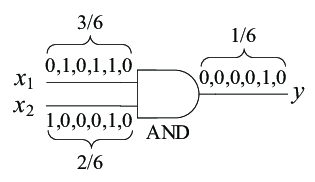
\includegraphics[scale=2]{pictures/mult.png}
\caption{Stochastic unipolar multiplication\cite{fig:multiplyslashadd}.}
\label{fig:multiplyslashadd}
\end{figure}
The above example shows a stochastic unipolar multiplication, the AND gate produces a 1 if both inputs contain a 1 else the output is 0. As shown in the example above in the 5th position both bitstream ($x_1$) and ($x_2$) contain a 1 so the output for the 5th position is also a 1.

The next example is a multiplication with the bipolar format using a XNOR gate which produces a 1 if both the inputs are the same ie (0 and 0) or (1 and 1) otherwise it produces a 0.
\begin{figure}[H]
\centering
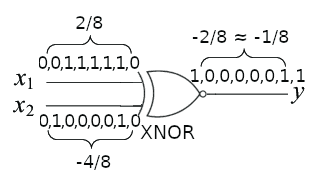
\includegraphics[scale=2]{pictures/mult_xnor.png}
\caption{Stochastic bipolar multiplication.}
\label{fig:multiplyslashaddbi}
\end{figure}

\section{Addition}
The last step of matrix multiplication is the addition, but this is the part where things didn't work out. So the first thing about stochastic addition is you cannot represent a number larger than what your stochastic range is, for example this means that you cannot represent a number larger than 1 if you are in a bipolar/unipolar format this means you have two forms of addition, saturating and non-saturating, in saturating addition it works similarly to normal addition with the exception that you cannot go over or under the limit (0/1 for unipolar, -1/1 for bipolar). In non-saturating addition, the resulting addition is divided by 2, this ensures that the stochastic number always stays within range.

However, the 2 caveats of stochastic addition leads to problems when trying to do matrix multiplication, starting the most common addition formation, non-saturating where a MUX gate is used as shown in the figure below.
\begin{figure}[H]
\centering
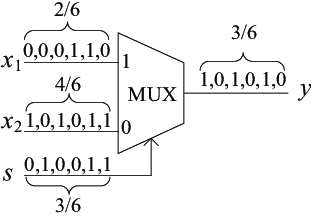
\includegraphics[scale=2]{pictures/add.png}
\caption{Stochastic unipolar non-saturating addition\cite{fig:multiplyslashadd}.}
\label{fig:multiplyslashadd}
\end{figure}
The MUX selects between the two incoming bitstreams with a probability of 50\% which translates to a result where the number is added together but scaled to always stay within the range of 0 to 1, ie $\frac{a+b}{2}$.

However, because of this division by 2, consecutive additions result in the number getting smaller and smaller with no way of recovering the original value.
If $a$,$b$,$c$ and $d$ are stochastic numbers then the non-saturating addition gets represented as,
$$\frac{\frac{\frac{a+b}{2}+c}{2}+d}{2} \neq a+b+c+d$$
An idea to get around this would be to premultiply each number beforehand such that the equation becomes
$$\frac{\frac{\frac{2a+2b}{2}+4c}{2}+8d}{2} = a+b+c+d$$
But the numbers get progressively larger by $2^x$ which would easily balloon out of hand for example if you have a 512 size array.

There is also another way of adding stochastic bitstreams and that is with the saturating addition which acts very much like a normal non-saturating addition. The saturating addition is simply an OR gate between the bitstreams  however the problem with this to do with the scale of the numbers used within a neural network, the floating-point numbers coming in from the previous layer in the neural network are normalized between 0 and 1 but these numbers can easily reach values that are smaller than 0.01 and representing really small numbers stochastic is not really doable without a high number of bits, even then the amount of bit required would easily exceed any systems memory and computation power. The other problem is the weights 

%\section{Alternate addition research}
%With the appeal of faster computing with stochastic computing, there has been quite a bit of research into how to get even more accurate results especially with an addition which tends to suffer from high accuracy loss. %TODO

\chapter{Results}

\subsection{Introduction}
In this section, I share some of the results and graphs I've made and talk about what this means in the context of my thesis.

\subsection{Unipolar multiplication accuracy}
This graph shows the multiplication of 2 stochastic bitstreams using a unipolar format with a varying bit-length (up to 10000 bits), the result of the multiplication should be $0.5*0.25=0.125$ as represented by the orange line.
\begin{figure}[H]
\centering
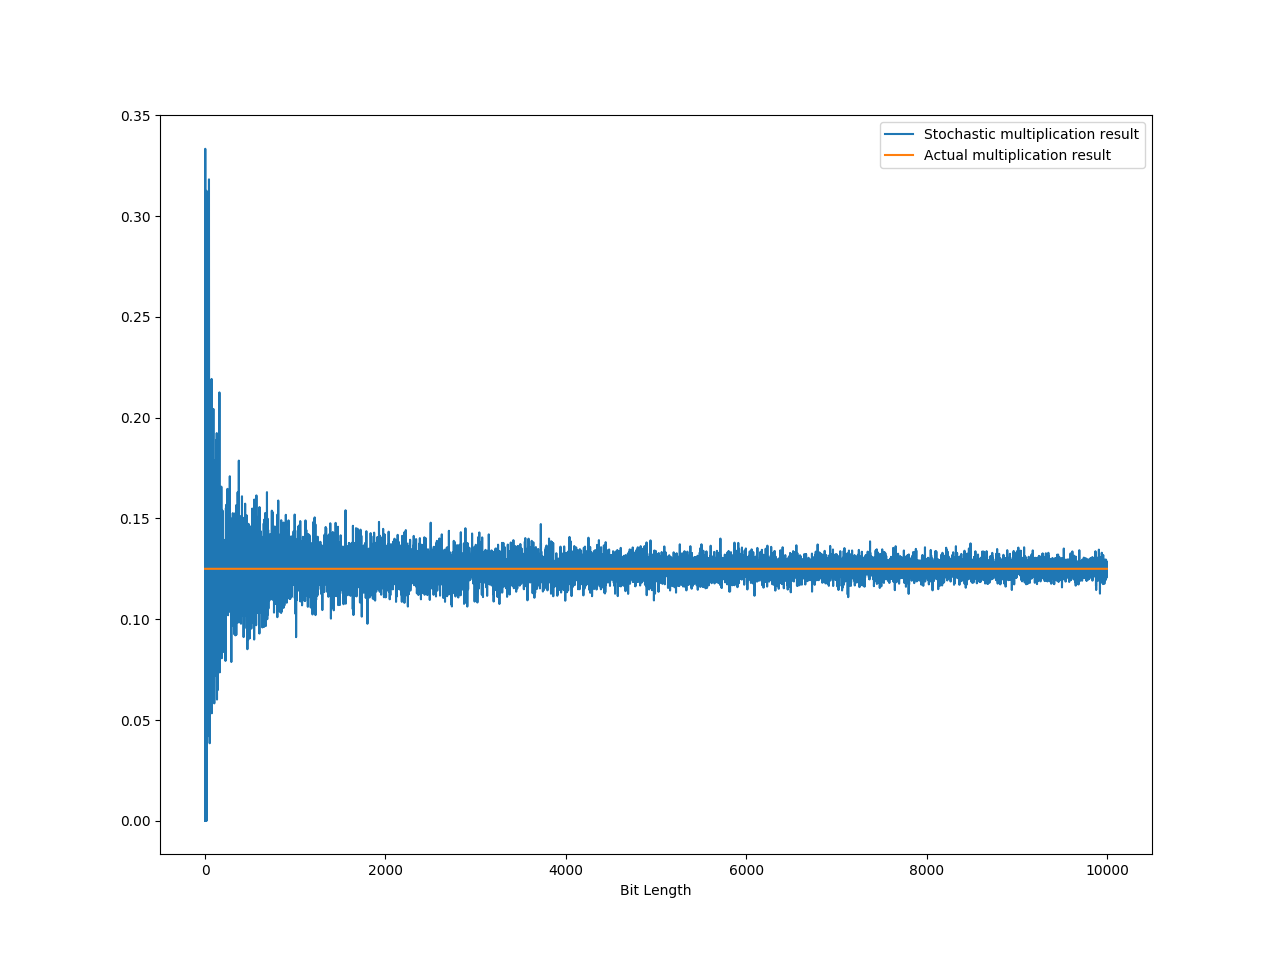
\includegraphics[scale=0.4]{results/Figure_1.png}
\caption{Stochastic multiplication.}
\label{fig:mult}
\end{figure}
\begin{figure}[H]
\centering
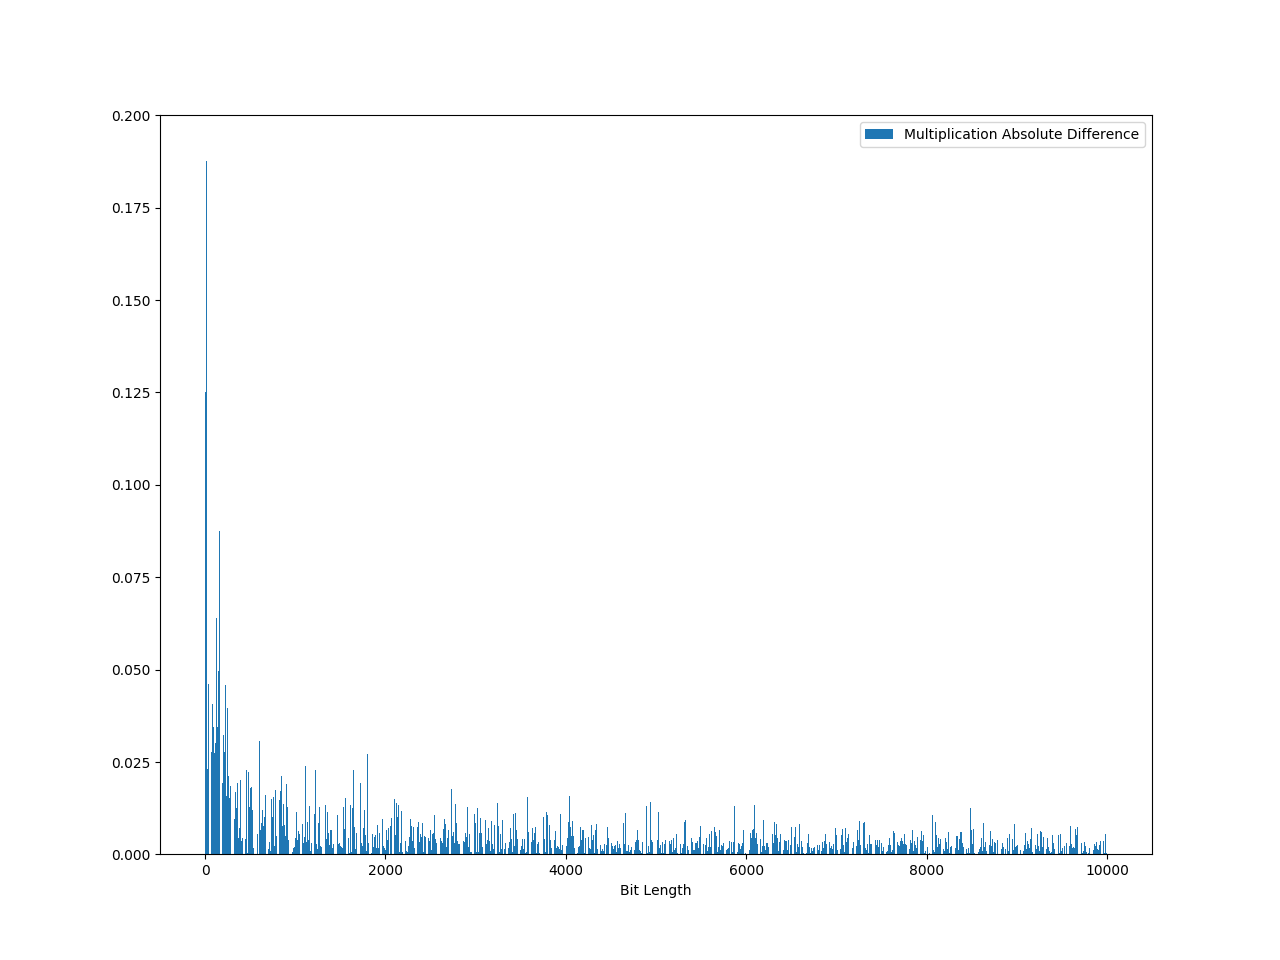
\includegraphics[scale=0.4]{results/Figure_1-abs.png}
\caption{Stochastic multiplication absolute difference.}
\label{fig:abs_mult}
\end{figure}
In the graphs above, we can see that as the length of the bitstream is increased the variance with the accuracy goes down but the gains are not linear and dropoff over time. The amount of accuracy needed to represent the ranges that a neural network uses would exceed 10000 bits.

\subsection{Bipolar multiplication accuracy}
This graph shows the multiplication of 2 stochastic bitstreams using a bipolar format with a varying bit-length (up to 10000 bits), the result of the multiplication should be $0.5*0.25=0.125$ as represented by the orange line.
\begin{figure}[H]
\centering
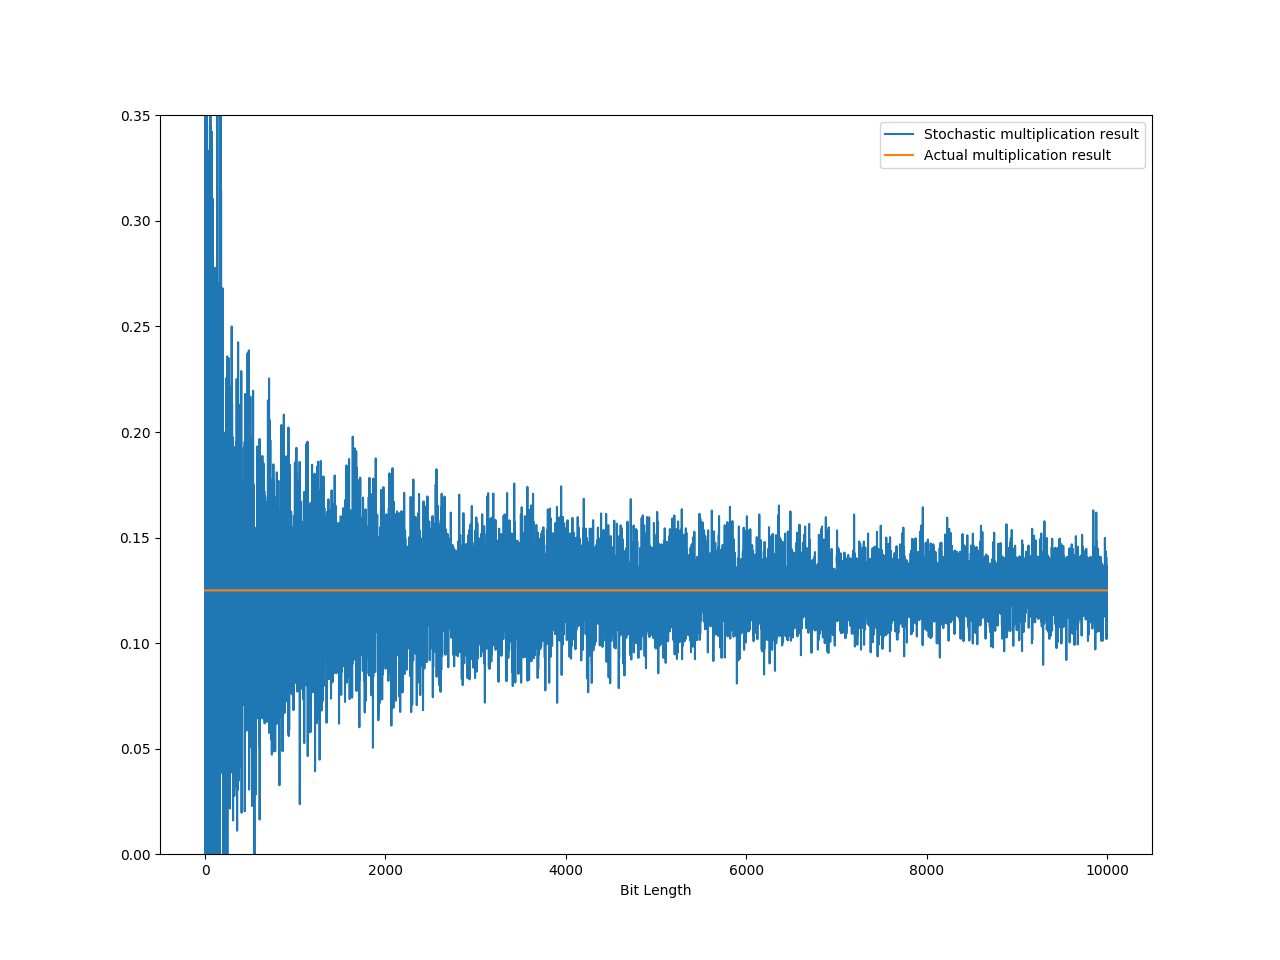
\includegraphics[scale=0.4]{results/Figure_1_bi.png}
\caption{Stochastic multiplication.}
\label{fig:mult}
\end{figure}
\begin{figure}[H]
\centering
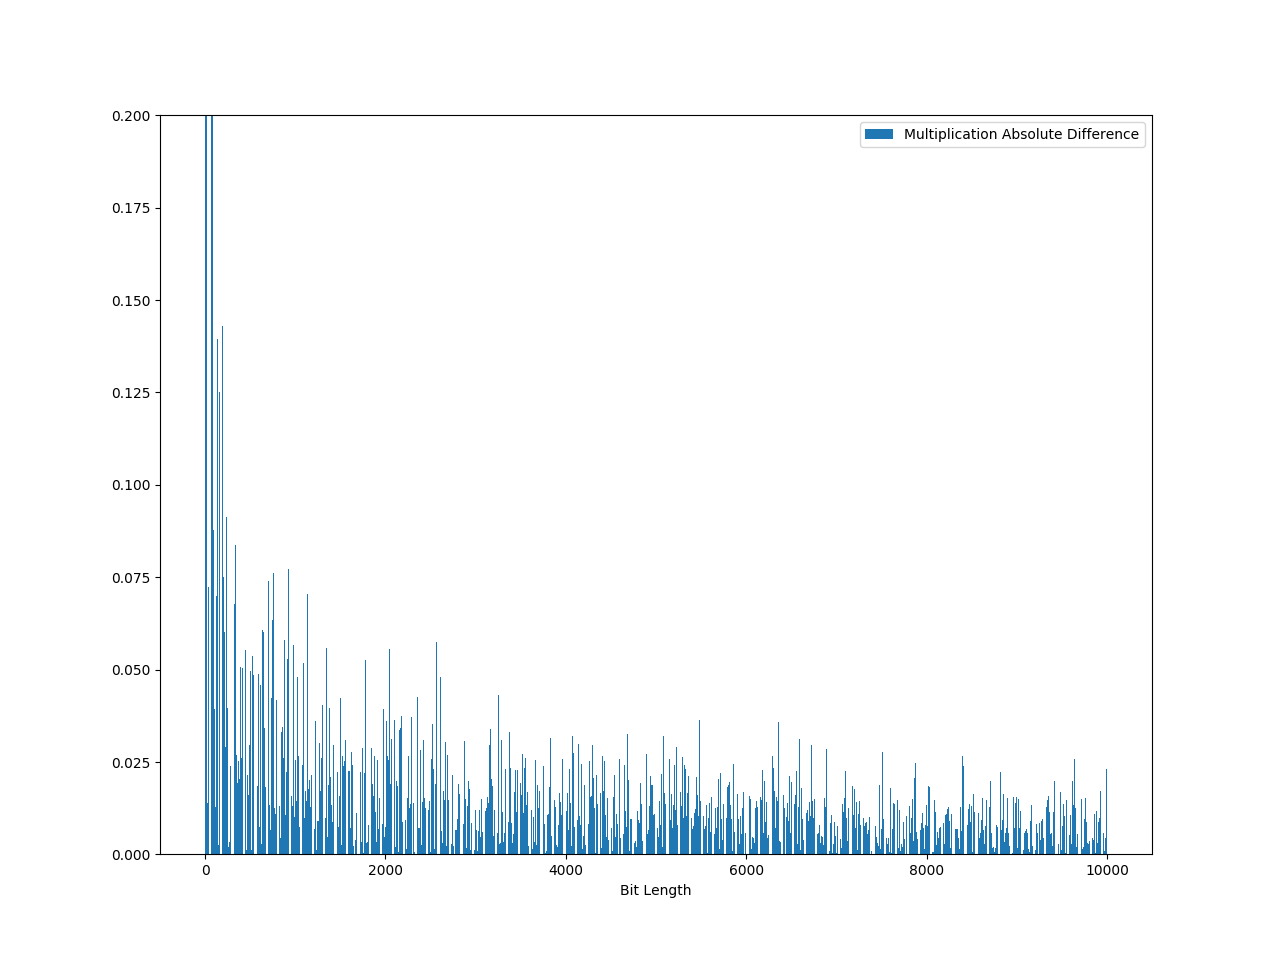
\includegraphics[scale=0.4]{results/Figure_1_bi_abs.png}
\caption{Stochastic multiplication absolute difference.}
\label{fig:abs_mult}
\end{figure}
When using a bipolar format the range is increased by a factor of 2 since instead of the range (0 to 1) we are now covering (-1 to 1) and when matched up at the same scale as the unipolar graph, we can see that the accuracy range has also increased, it becomes even more obvious when we look at the absolute values which have much larger spikes than the unipolar format.

\subsection{Non saturating addition accuracy}
This graph shows the addition of 2 stochastic bitstreams using the non-saturating addition with a varying bit-length (up to 10000 bits), the result of the multiplication should be $0.5*(0.5+0.25)=0.375$ as represented by the orange line.

\begin{figure}[H]
\centering
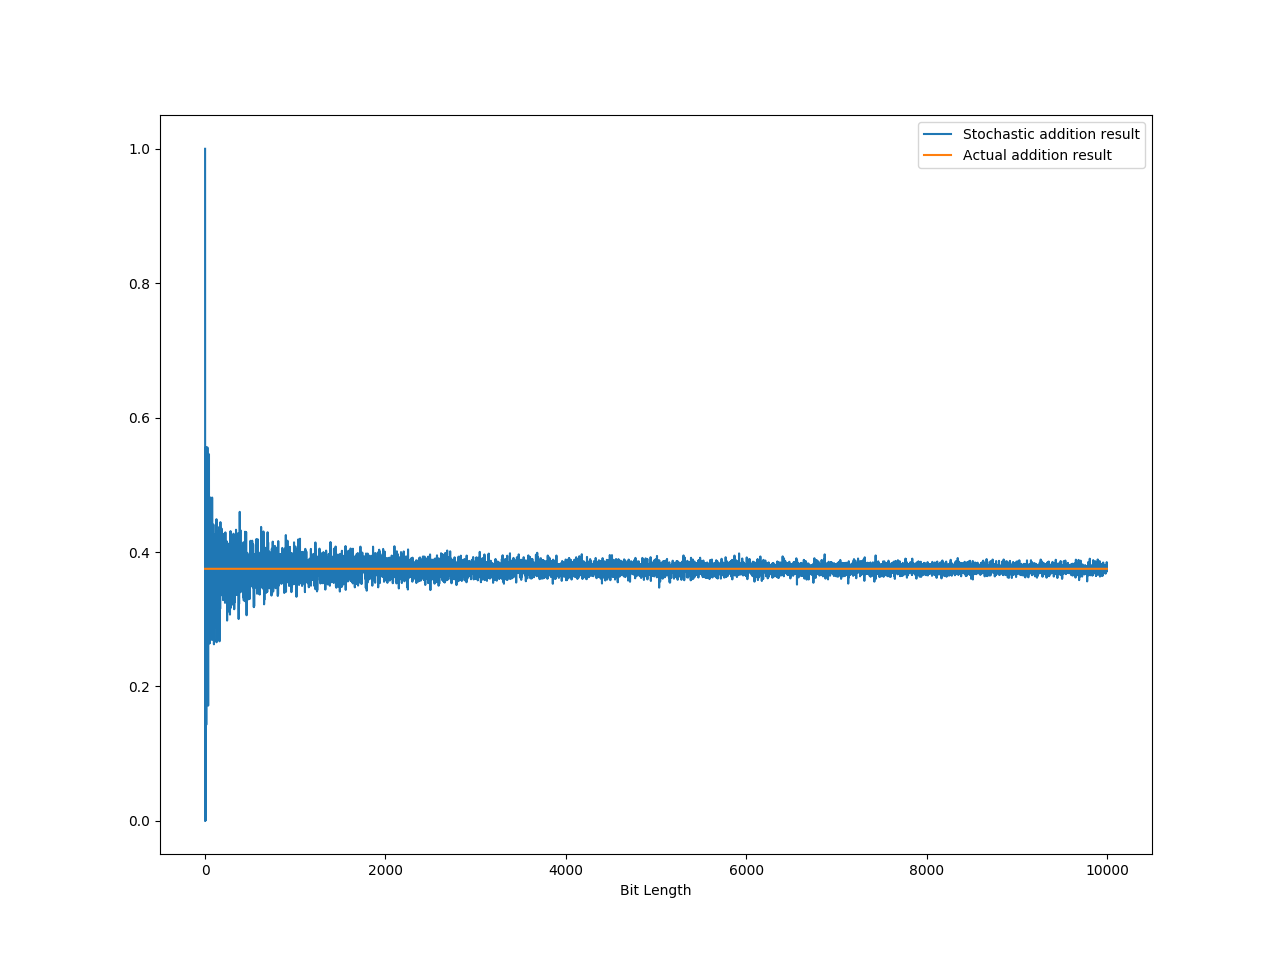
\includegraphics[scale=0.4]{results/Figure_2.png}
\label{fig:no_sat}
\caption{Non saturating stochastic addition.}
\end{figure}
\begin{figure}[H]
\centering
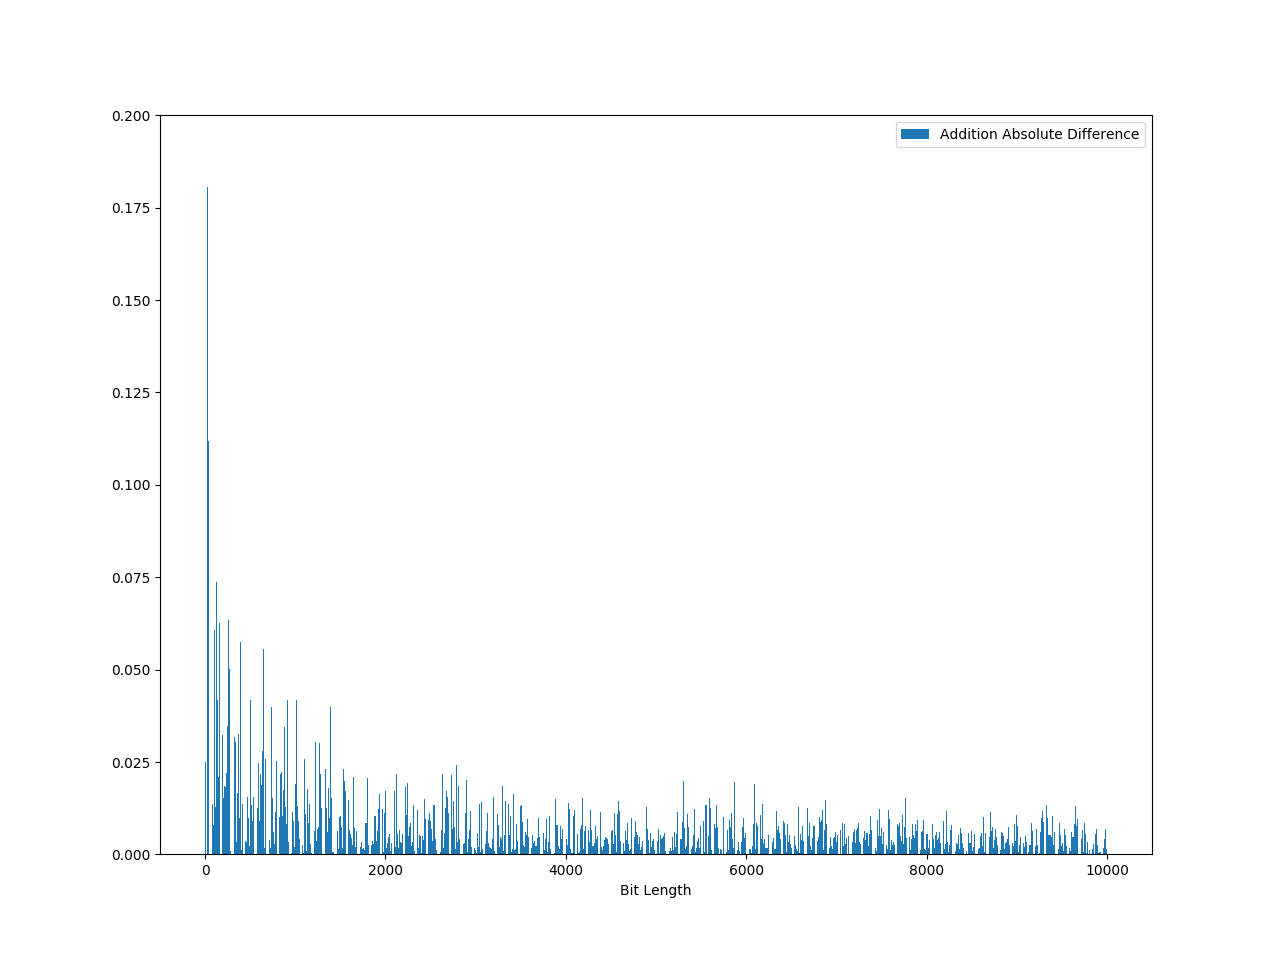
\includegraphics[scale=0.4]{results/Figure_2-abs.png}
\label{fig:abs_no_sat}
\caption{Non saturating stochastic addition absolute difference.}
\end{figure}
Similar to multiplication, non-saturating additions accuracy variance goes down with the number of bits but it also has the same issue with the gains in accuracy dropping off over time. Fortunately, the addition seems to have slightly better accuracy than multiplication but not by much.

\subsection{Saturating addition accuracy}
This graph shows the addition of 2 stochastic bitstreams using saturating addition with a varying bit-length (up to 10000 bits), the first graph should show the addition of $0.5+0.25=0.75$

\begin{figure}[H]
\centering
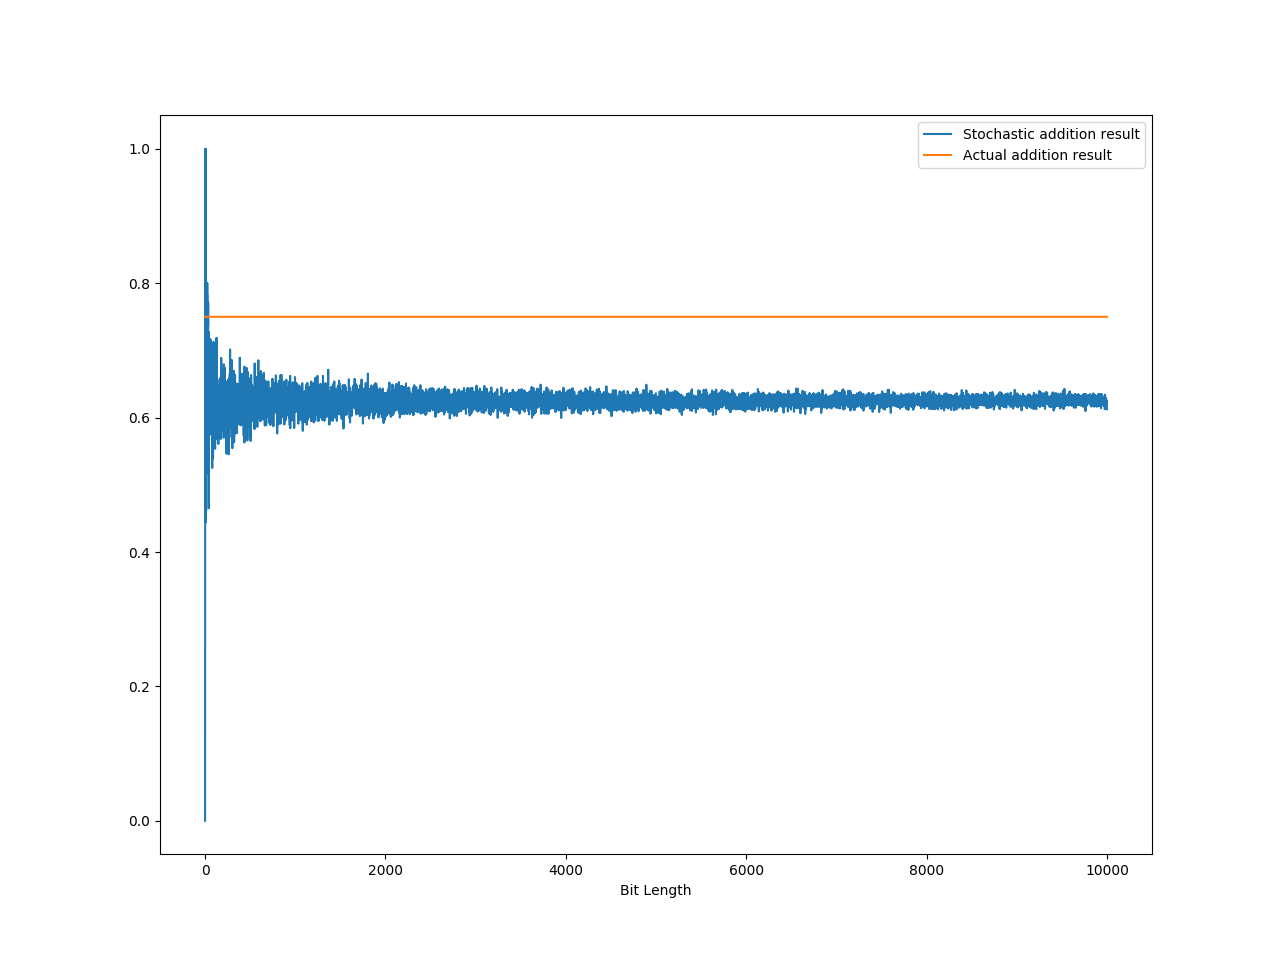
\includegraphics[scale=0.4]{results/Figure_3.png}
\caption{Saturating stochastic addition.}
\label{fig:sat_add}
\end{figure}
Saturating addition has the advantage of not trying to restrict the range of the addition which is useful in repeated additions for matrix multiplications however what was found was that saturating additions seems to have an offset from the intended target which increases as the result is closer to 1. The graphs below should demonstrate my point,
\begin{figure}[H]
\centering
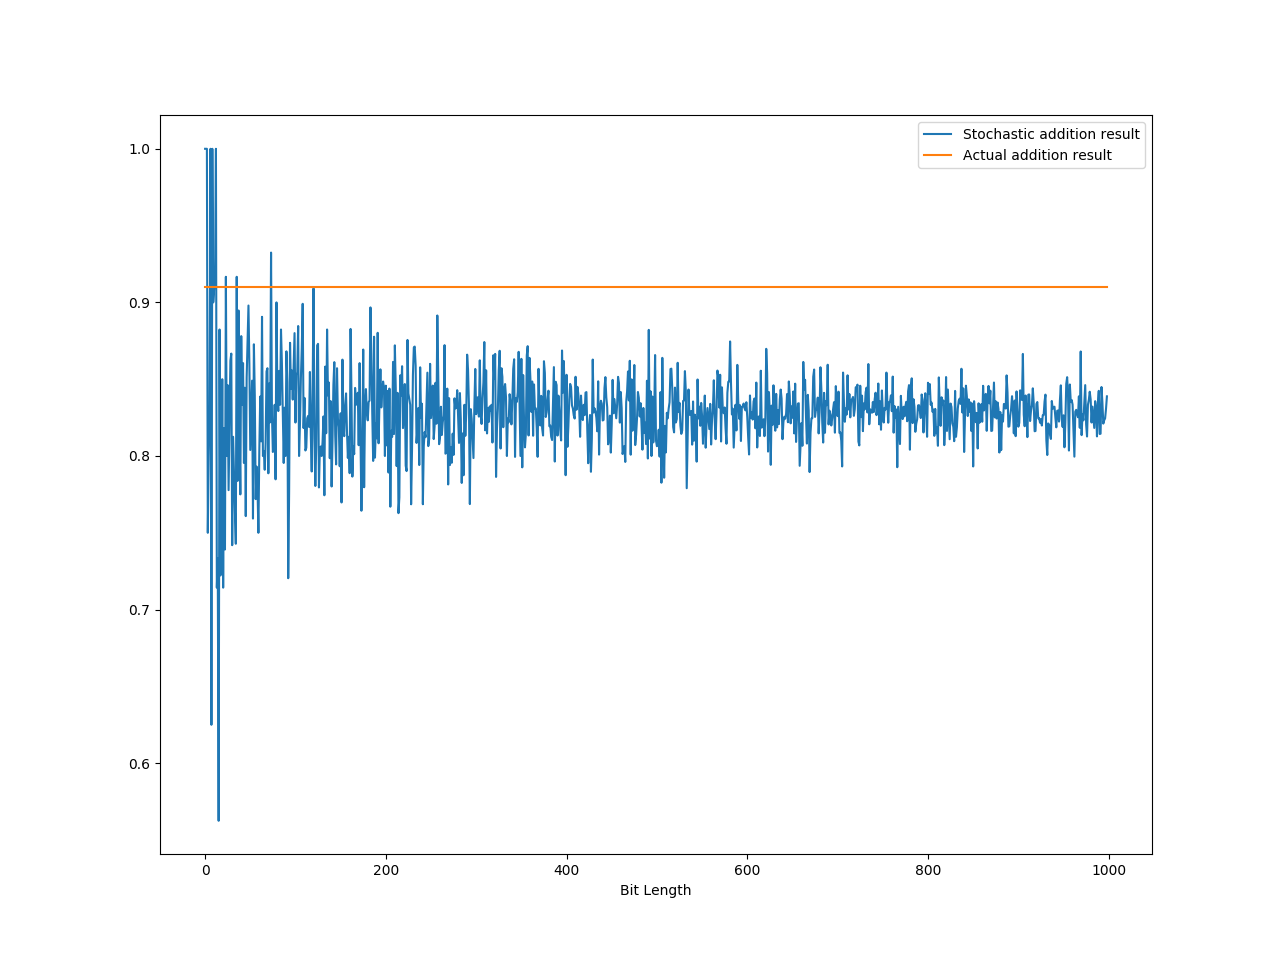
\includegraphics[scale=0.4]{results/Figure_3_high.png}
\caption{Saturating stochastic addition high values.}
\label{fig:sat_high}
\end{figure}
\begin{figure}[H]
\centering
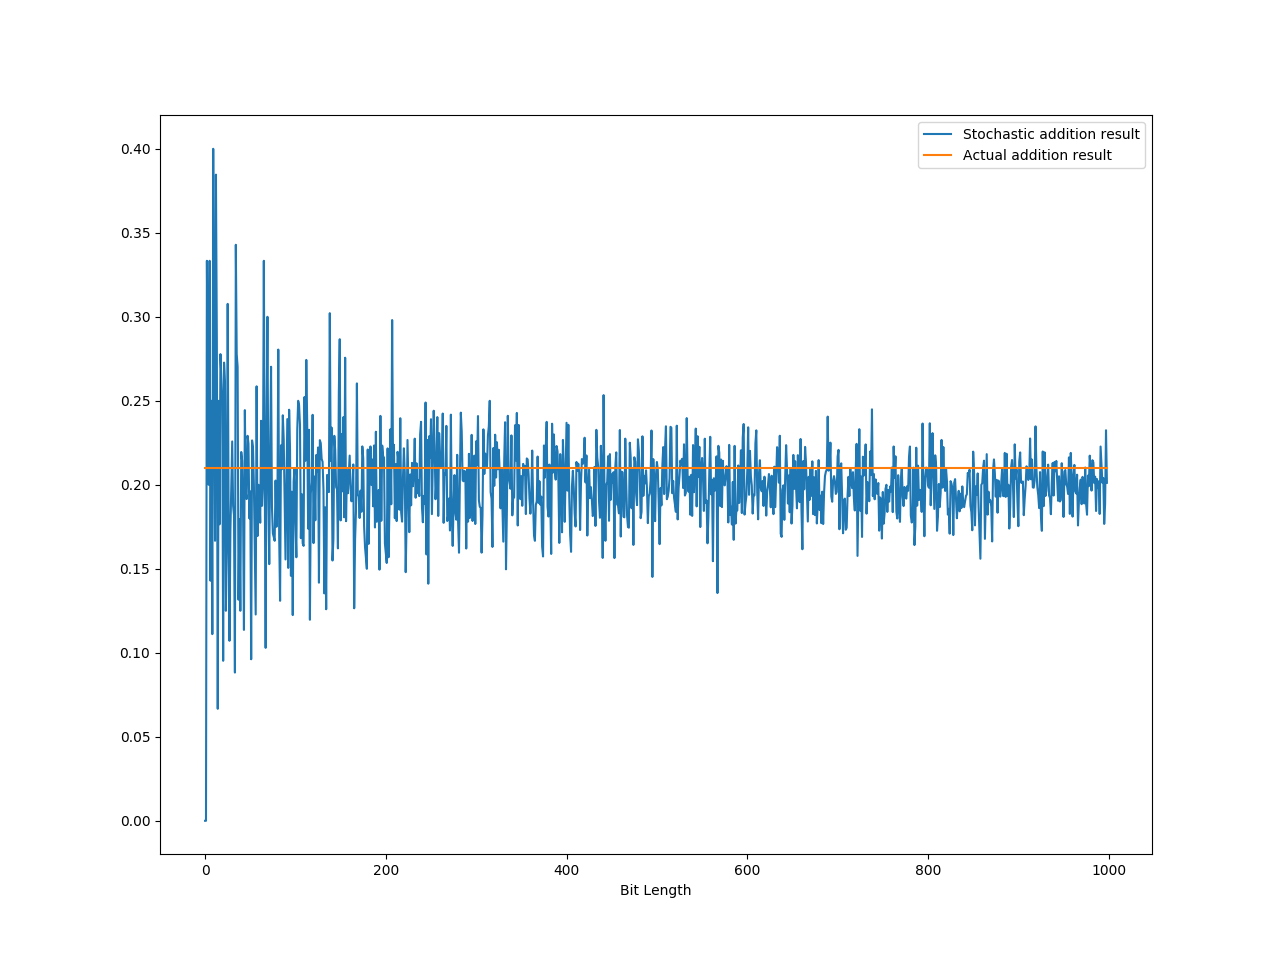
\includegraphics[scale=0.4]{results/Figure_3_low.png}
\caption{Saturating stochastic addition low values.}
\label{fig:sat_low}
\end{figure}

In the first graph, the resulting addition should be $0.81+0.1=0.91$ but the stochastic addition is offset by around $0.8$ but in the second graph there is a much lower offset of around $0.02$. To demonstrate my point further, I've fixed the bitlength to a 1000 bits, changing only the result of the addition.

\begin{figure}[H]
\centering
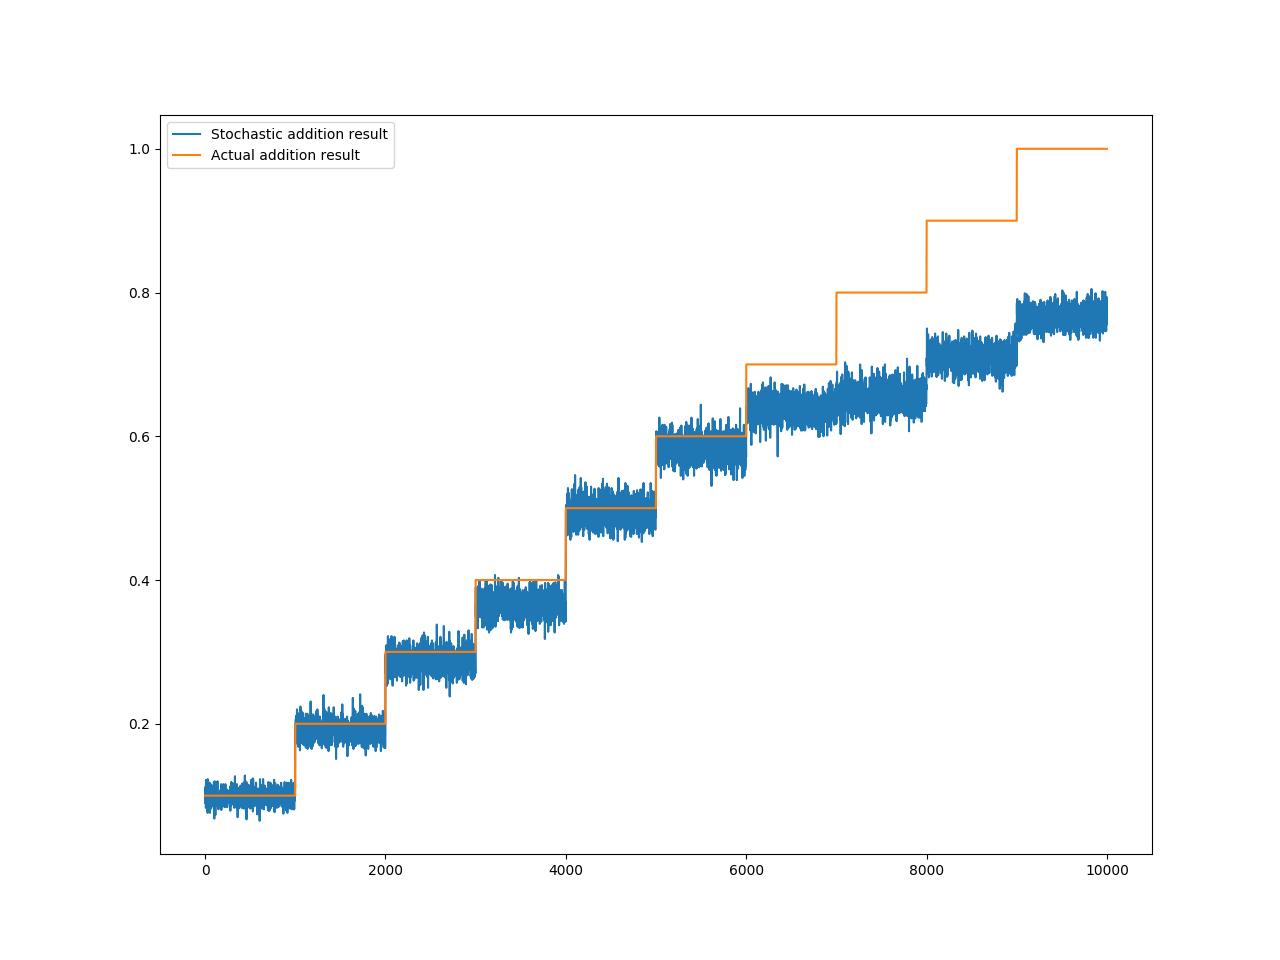
\includegraphics[scale=0.4]{results/Figure_3_sss.png}
\caption{Stochastic stochastic addition multiple values.}
\label{fig:sat_add_multiple}
\end{figure}
As a result of the addition approaches 1, the addition becomes offset from the target by an ever-increasing amount. This seems to match up closely with an algorithmic anaylsis of stochastic computing which states that a saturating addition computes to $X = a+b-ab$\cite{logic-gates}, such that when $a$ and $b$ becomes larger so does $ab$.

\subsection{Spliting the bitstream}
One of the proposals to get around the limitations the accuracy of stochastic bitstreams was to split the bitstream into two parts, one containing the decimal part and the other containing the integer component. The idea behind splitting the bitstream into two parts was to keep the high accuracy for the decimal part and because of the integer component only being composed of whole numbers we could use a smaller bitstream length to represent more integers and gain more accuracy, this is especially relevant when considering the diminishing returns on increasing the bitstream for more accuracy.
\begin{figure}[H]
\centering
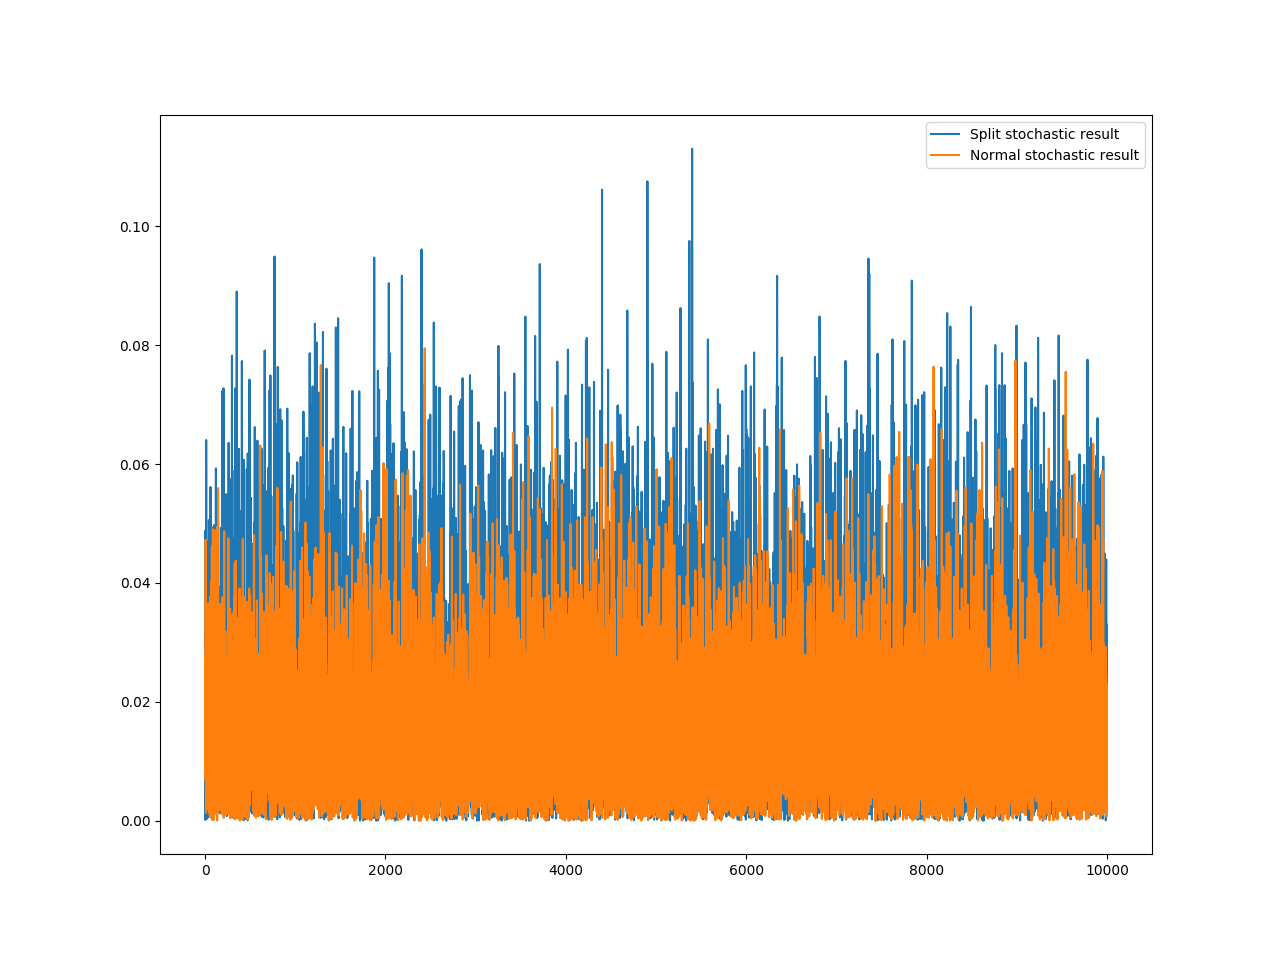
\includegraphics[scale=0.4]{results/Figure_4.png}
\caption{Spliting the bitstream (addition).}
\label{fig:spliting}
\end{figure}
The figure above shows a stochastic addition with the absolute difference between the result and the intended result, the method where the bitstream is split into 2 parts shows a higher absolute difference and thus is less accurate than the normal non-splitting method. This is the same with multiplication as shown in the figure below.
\begin{figure}[H]
\centering
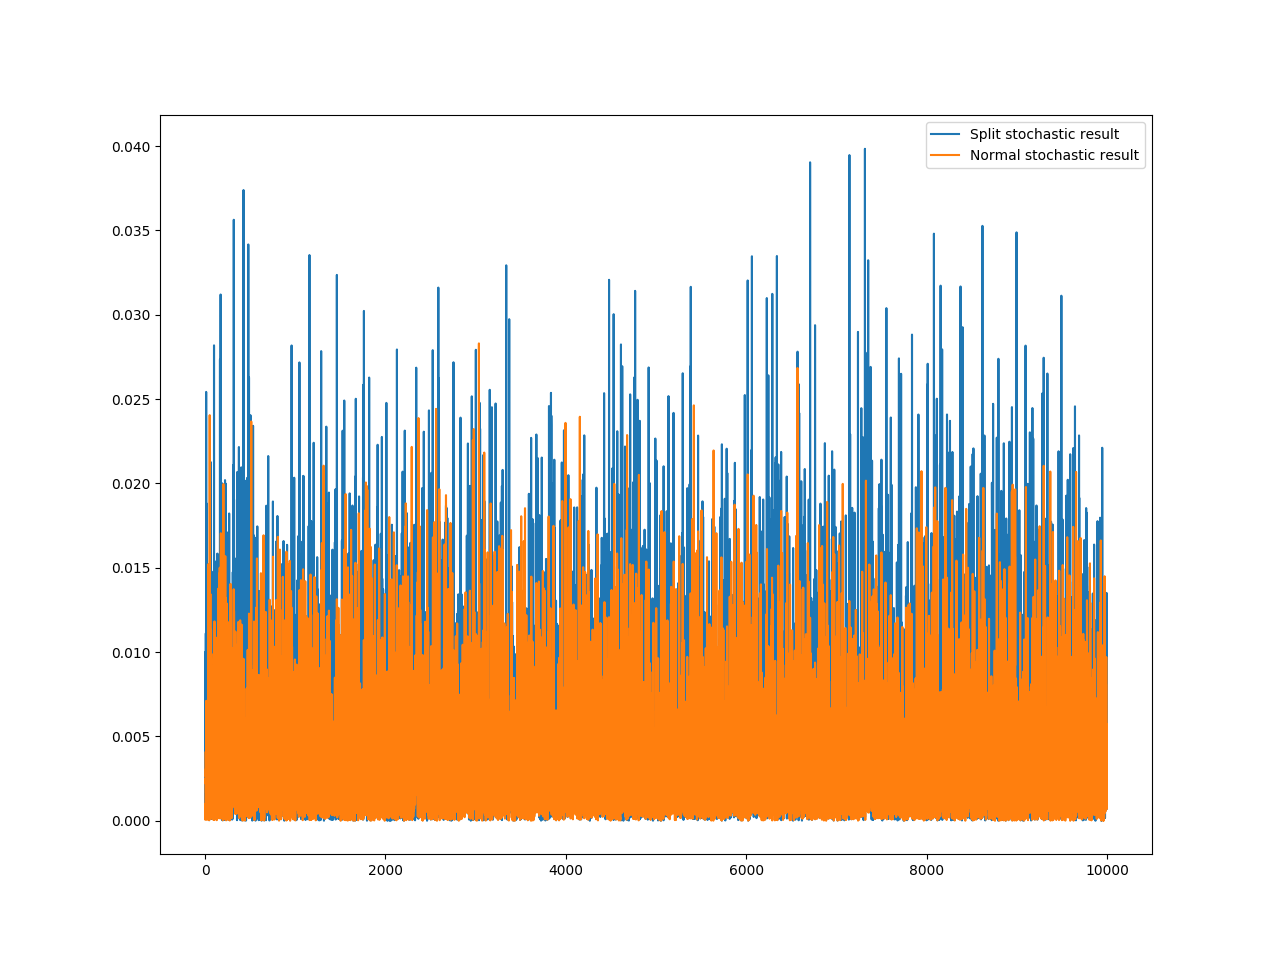
\includegraphics[scale=0.4]{results/Figure_5.png}
\caption{Spliting the bitstream (multiplication).}
\label{fig:spliting}
\end{figure}

\chapter{Future Work}
The current design I have proposed has certain limitations and bounds that make it suitable for application regarding machine learning, as such this section will describe, future work to try and accomplish this goal as well as describing a theoretical device that would be able to work with neural networks.

\subsection{Limitation 1}
The first limitation of my design is the memory limits, as I'm emulating a stochastic bitstream, each number in the matrix gets expanded out and this can easily exceed memory limits. The solution to this a way of a restructuring of the machine learning framework to accept a stream of data, this way only a few bits are being processed at a time. The difficulty here is that machine learning frameworks are not based around the idea of streaming data, batches of data are loaded onto the GPU and processed but this is at a very low level and it is very likely you would need to heavily restructure the machine learning framework, which is where a secondary problem comes in which is by modifying the machine learning framework to work with streams it becomes very hard to compare 2 results (other than raw accuracy) with each other as the calculations have changed and are no longer 1 to 1 comparable.

\subsection{Limitation 2}
The second limitation of my design is which has made it impossible to get results, is the acceptable range of the stochastic matrix. Due to the nature of stochastic numbers as to how they are simply a probability, each stochastic number has a range from 0 to 1, this can be mapped to other ranges after converting it back to a floating-point but when it is within a stochastic number the range is limited. Due to this limitation, my implementation of matrix multiplication can only do matrix multiplication where the final range is between 0 and 1 or where the final range of the matrix multiplication is known and can be mapped afterwards.

\subsection{Theoretical device}
Regarding the future work of this thesis, the neural network has to be built from the ground up using a stream-based idea. The multiplication and addition will need to be separate units which are then chained together to create the final solution. In addition to this, the addition problem regarding the range of the stochastic numbers will need an alternative solution with fewer drawbacks. In reality the stochastic numbers cannot really be thought of as just floating-point numbers of integer binary point numbers, in reality, they are more arbitrary point numbers and the larger amount of bits processed the surer you are of the answer, maybe a concept to look into is quantum computers as they also work on the idea of probabilities.

\chapter{Conclusions}
\label{chap:Conclusions}

\section{Conclusions}
\label{sec:ConclusionsConclusions}
In conclusion, trying to apply stochastic computing to the field of machine learning through matrix operations alone is unlikely to succeed. Stochastic computing needs a lot more groundwork, regarding the inaccuracy and range limitation to be used outside its field and for stochastic computing to be able to be fully integrated with machine learning there will need to be a large paradigm shift in how they are used and applied.

\clearemptydoublepage
\chapter{Abbreviations}
\label{chap:abbreviations}

\begin{tabbing}

AWGN \qquad \qquad \= Additive White Gaussian Noise\\
SGD \> Stochastic Gradient Descent\\
SC \> Stochastic numbers\\
NN \> Neural network \\
MLP \> Multi Layer Perceptron \\
CNN \> Convolutional neural network \\
RNN \> Recurrent neural network \\
RELU \> Rectified linear unit \\
MNIST \> Modified National Institute of Standards and Technology \\
CIFAR \> Canadian Institute For Advanced Research \\
\end{tabbing}

%\phantomsection \addcontentsline{toc}{chapter}{Index}
% \renewcommand{\baselinestretch}{1} \small \normalsize
% \printindex

\appendix
\section{Codebase and results}
\url{https://github.com/AeroX2/stochastic-demo}

%\input{Bibliography/biblio3}
\bibliographystyle{IEEEtranS}
%\bibliographystyle{acm}
\bibliography{my_reference}
%\bibliography{Bibliography/biblio4}

\end{document}


